\section{日期函数}
\subsection{YEAR、MONTH 和 DAY函数}

YEAR：返回对应于某个日期的年份。 Year 作为 1900 - 9999 之间的整数返回。

MONTH：返回日期中的月份。 月份是介于 1（一月）到 12（十二月）之间的整数。

DAY：返回以序列数表示的某日期的天数。 天数是介于 1 到 31 之间的整数。

=YEAR(A3)

=YEAR(``2022/11/14'')

=YEAR(``2022-11-14'')

\begin{itemize}
    \item 当直接在函数中输入日期时，您需要将其用引号引起。
    \item Microsoft Excel 可将日期存储为可用于计算的序列号。 默认情况下，1900 年 1 月 1 日的序列号是 1，而 2008 年 1 月 1 日的序列号是 39448，这是因为它距 1900 年 1 月 1 日有 39448 天。
    \item 无论提供的日期值的显示格式如何，YEAR、MONTH 和 DAY 函数返回的值都是公历值。 例如，如果提供的日期的显示格式是农历，则 YEAR、MONTH 和 DAY 函数返回的值将是与对应的公历日期相关联的值。
\end{itemize}

\subsection{TODAY函数}

返回当前日期的序列号。

语法：

TODAY()

TODAY 函数语法没有参数。

不管您何时打开工作薄，当需要在工作表上显示当前日期时，TODAY 函数非常有用。 

它还可用于计算时间间隔。 例如，如果您知道某人出生于 1963 年，您可使用以下公式计算对方到其今年生日为止的年龄：

= YEAR(TODAY())-1963

\subsection{DATE函数}

如果需要采用三个单独的值并将它们合并为一个日期，请使用DATE 函数。

语法：DATE(year,month,day)

\begin{itemize}
    \item Year 必需。默认情况下，Excel使用 1900 日期系统，这意味着第一个日期是 1900 年 1 月 1 日。
        \begin{itemize}
            \item 如果 year 介于 0（零）到 1899 之间（包含这两个值），则 Excel 会将该值与 1900 相加来计算年份。 例如，DATE(108,1,2) 返回 2008 年 1 月 2 日 (1900+108)。
            \item 如果 year 介于 1900 到 9999 之间（包含这两个值），则 Excel 将使用该数值作为年份。 
            \item 如果 year 小于 0 或大于 10000，Excel 将返回\#NUM！ 错误值。
        \end{itemize}
    \item Month 必需。
        \begin{itemize}
            \item 如果month大于12，则month会从指定年份的第一个月开始加上该月份数。 例如，DATE(2008,14,2) 返回表示 2009 年 2 月 2 日的序列数。
            \item 如果 month 小于 1，则 month 会从指定年份的第一个月开始减去该月份数，然后再加上 1 个月。 例如，DATE(2008,-3,2) 返回表示 2007 年 9 月 2 日的序列号。
        \end{itemize}
    \item Day 必需。
        \begin{itemize}
            \item 如果 day 大于指定月中的天数，则 day 会从该月的第一天开始加上该天数。 例如，DATE(2008,1,35) 返回表示 2008 年 2 月 4 日的序列数。
            \item 如果 day 小于 1，则 day 从指定月份的第一天开始减去该天数，然后再加上 1 天。 例如，DATE(2008,1,-15) 返回表示 2007 年 12 月 16 日的序列号。
        \end{itemize}
\end{itemize}


\subsection{更改日期格式}

当您在单元格中输入一些文本（如``2/2''）时，Excel 会假定这是日期，并且根据``控制面板''中的默认日期设置设置格式。

更改日期格式：右键单击要更改的单元格，设置单元格格式或者按 Ctrl+1

\begin{figure}[htpb]
    \centering
    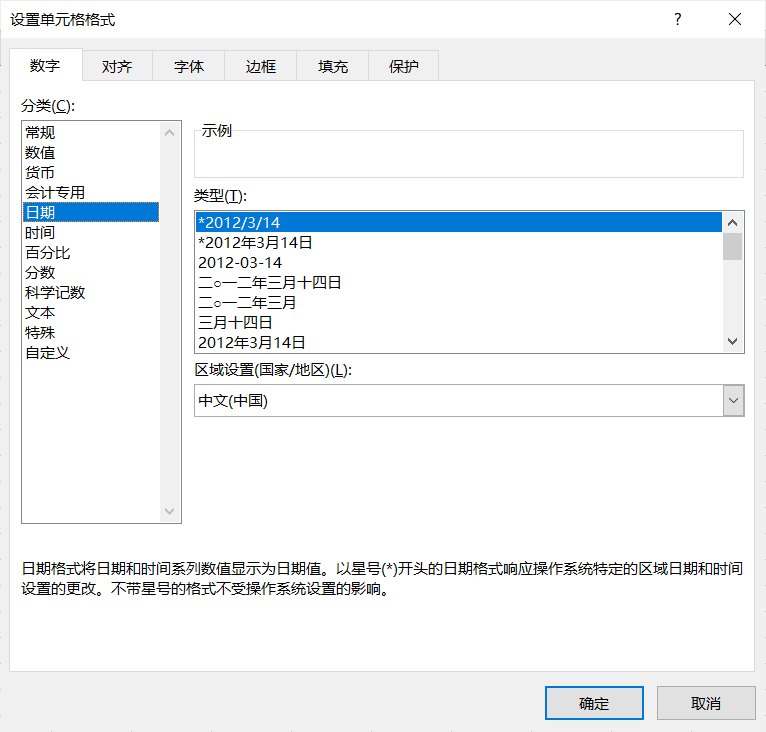
\includegraphics[width=.6\linewidth]{figures/date.png}
\end{figure}

单元格中的数字是否显示为 \#\#\#\#\#？ 单元格可能不够宽，无法显示整个数字。 请尝试双击含 \#\#\#\#\# 单元格的列的右边界。 这样可以重新调整列的大小，使其适应数字。 您也可以拖动列的右边界，以使列达到所需的大小。

\subsection{时间函数}

HOUR：返回时间的小时数，小时数是介于 0 到 23 之间的整数。

MINUTE：返回时间的分钟数，分钟是一个介于 0 到 59 之间的整数。

SECOND：返回时间的秒数，秒数是 0到 59 范围内的整数。

Now()：返回当前日期和时间的序列号。NOW 函数语法没有参数。

TIME：返回特定时间的十进制数字。 如果在输入该函数之前单元格格式为``常规''，则结果将使用日期格式。

TIME(hour, minute, second)

Excel 将每 24 小时的周期作为一个从 0 至 1（不包括 1）的小数存储。

由 TIME 返回的十进制数字是一个范围在 0（零）到 0.999988426 之间的值，表示 0:00:00 (12:00:00 AM) 到 23:59:59 (11:59:59 P.M.) 之间的时间。